% Options for packages loaded elsewhere
\PassOptionsToPackage{unicode}{hyperref}
\PassOptionsToPackage{hyphens}{url}
\PassOptionsToPackage{dvipsnames,svgnames,x11names}{xcolor}
%
\documentclass[
  letterpaper,
  DIV=11,
  numbers=noendperiod]{scrartcl}

\usepackage{amsmath,amssymb}
\usepackage{iftex}
\ifPDFTeX
  \usepackage[T1]{fontenc}
  \usepackage[utf8]{inputenc}
  \usepackage{textcomp} % provide euro and other symbols
\else % if luatex or xetex
  \usepackage{unicode-math}
  \defaultfontfeatures{Scale=MatchLowercase}
  \defaultfontfeatures[\rmfamily]{Ligatures=TeX,Scale=1}
\fi
\usepackage{lmodern}
\ifPDFTeX\else  
    % xetex/luatex font selection
\fi
% Use upquote if available, for straight quotes in verbatim environments
\IfFileExists{upquote.sty}{\usepackage{upquote}}{}
\IfFileExists{microtype.sty}{% use microtype if available
  \usepackage[]{microtype}
  \UseMicrotypeSet[protrusion]{basicmath} % disable protrusion for tt fonts
}{}
\makeatletter
\@ifundefined{KOMAClassName}{% if non-KOMA class
  \IfFileExists{parskip.sty}{%
    \usepackage{parskip}
  }{% else
    \setlength{\parindent}{0pt}
    \setlength{\parskip}{6pt plus 2pt minus 1pt}}
}{% if KOMA class
  \KOMAoptions{parskip=half}}
\makeatother
\usepackage{xcolor}
\setlength{\emergencystretch}{3em} % prevent overfull lines
\setcounter{secnumdepth}{-\maxdimen} % remove section numbering
% Make \paragraph and \subparagraph free-standing
\makeatletter
\ifx\paragraph\undefined\else
  \let\oldparagraph\paragraph
  \renewcommand{\paragraph}{
    \@ifstar
      \xxxParagraphStar
      \xxxParagraphNoStar
  }
  \newcommand{\xxxParagraphStar}[1]{\oldparagraph*{#1}\mbox{}}
  \newcommand{\xxxParagraphNoStar}[1]{\oldparagraph{#1}\mbox{}}
\fi
\ifx\subparagraph\undefined\else
  \let\oldsubparagraph\subparagraph
  \renewcommand{\subparagraph}{
    \@ifstar
      \xxxSubParagraphStar
      \xxxSubParagraphNoStar
  }
  \newcommand{\xxxSubParagraphStar}[1]{\oldsubparagraph*{#1}\mbox{}}
  \newcommand{\xxxSubParagraphNoStar}[1]{\oldsubparagraph{#1}\mbox{}}
\fi
\makeatother

\usepackage{color}
\usepackage{fancyvrb}
\newcommand{\VerbBar}{|}
\newcommand{\VERB}{\Verb[commandchars=\\\{\}]}
\DefineVerbatimEnvironment{Highlighting}{Verbatim}{commandchars=\\\{\}}
% Add ',fontsize=\small' for more characters per line
\usepackage{framed}
\definecolor{shadecolor}{RGB}{241,243,245}
\newenvironment{Shaded}{\begin{snugshade}}{\end{snugshade}}
\newcommand{\AlertTok}[1]{\textcolor[rgb]{0.68,0.00,0.00}{#1}}
\newcommand{\AnnotationTok}[1]{\textcolor[rgb]{0.37,0.37,0.37}{#1}}
\newcommand{\AttributeTok}[1]{\textcolor[rgb]{0.40,0.45,0.13}{#1}}
\newcommand{\BaseNTok}[1]{\textcolor[rgb]{0.68,0.00,0.00}{#1}}
\newcommand{\BuiltInTok}[1]{\textcolor[rgb]{0.00,0.23,0.31}{#1}}
\newcommand{\CharTok}[1]{\textcolor[rgb]{0.13,0.47,0.30}{#1}}
\newcommand{\CommentTok}[1]{\textcolor[rgb]{0.37,0.37,0.37}{#1}}
\newcommand{\CommentVarTok}[1]{\textcolor[rgb]{0.37,0.37,0.37}{\textit{#1}}}
\newcommand{\ConstantTok}[1]{\textcolor[rgb]{0.56,0.35,0.01}{#1}}
\newcommand{\ControlFlowTok}[1]{\textcolor[rgb]{0.00,0.23,0.31}{\textbf{#1}}}
\newcommand{\DataTypeTok}[1]{\textcolor[rgb]{0.68,0.00,0.00}{#1}}
\newcommand{\DecValTok}[1]{\textcolor[rgb]{0.68,0.00,0.00}{#1}}
\newcommand{\DocumentationTok}[1]{\textcolor[rgb]{0.37,0.37,0.37}{\textit{#1}}}
\newcommand{\ErrorTok}[1]{\textcolor[rgb]{0.68,0.00,0.00}{#1}}
\newcommand{\ExtensionTok}[1]{\textcolor[rgb]{0.00,0.23,0.31}{#1}}
\newcommand{\FloatTok}[1]{\textcolor[rgb]{0.68,0.00,0.00}{#1}}
\newcommand{\FunctionTok}[1]{\textcolor[rgb]{0.28,0.35,0.67}{#1}}
\newcommand{\ImportTok}[1]{\textcolor[rgb]{0.00,0.46,0.62}{#1}}
\newcommand{\InformationTok}[1]{\textcolor[rgb]{0.37,0.37,0.37}{#1}}
\newcommand{\KeywordTok}[1]{\textcolor[rgb]{0.00,0.23,0.31}{\textbf{#1}}}
\newcommand{\NormalTok}[1]{\textcolor[rgb]{0.00,0.23,0.31}{#1}}
\newcommand{\OperatorTok}[1]{\textcolor[rgb]{0.37,0.37,0.37}{#1}}
\newcommand{\OtherTok}[1]{\textcolor[rgb]{0.00,0.23,0.31}{#1}}
\newcommand{\PreprocessorTok}[1]{\textcolor[rgb]{0.68,0.00,0.00}{#1}}
\newcommand{\RegionMarkerTok}[1]{\textcolor[rgb]{0.00,0.23,0.31}{#1}}
\newcommand{\SpecialCharTok}[1]{\textcolor[rgb]{0.37,0.37,0.37}{#1}}
\newcommand{\SpecialStringTok}[1]{\textcolor[rgb]{0.13,0.47,0.30}{#1}}
\newcommand{\StringTok}[1]{\textcolor[rgb]{0.13,0.47,0.30}{#1}}
\newcommand{\VariableTok}[1]{\textcolor[rgb]{0.07,0.07,0.07}{#1}}
\newcommand{\VerbatimStringTok}[1]{\textcolor[rgb]{0.13,0.47,0.30}{#1}}
\newcommand{\WarningTok}[1]{\textcolor[rgb]{0.37,0.37,0.37}{\textit{#1}}}

\providecommand{\tightlist}{%
  \setlength{\itemsep}{0pt}\setlength{\parskip}{0pt}}\usepackage{longtable,booktabs,array}
\usepackage{calc} % for calculating minipage widths
% Correct order of tables after \paragraph or \subparagraph
\usepackage{etoolbox}
\makeatletter
\patchcmd\longtable{\par}{\if@noskipsec\mbox{}\fi\par}{}{}
\makeatother
% Allow footnotes in longtable head/foot
\IfFileExists{footnotehyper.sty}{\usepackage{footnotehyper}}{\usepackage{footnote}}
\makesavenoteenv{longtable}
\usepackage{graphicx}
\makeatletter
\newsavebox\pandoc@box
\newcommand*\pandocbounded[1]{% scales image to fit in text height/width
  \sbox\pandoc@box{#1}%
  \Gscale@div\@tempa{\textheight}{\dimexpr\ht\pandoc@box+\dp\pandoc@box\relax}%
  \Gscale@div\@tempb{\linewidth}{\wd\pandoc@box}%
  \ifdim\@tempb\p@<\@tempa\p@\let\@tempa\@tempb\fi% select the smaller of both
  \ifdim\@tempa\p@<\p@\scalebox{\@tempa}{\usebox\pandoc@box}%
  \else\usebox{\pandoc@box}%
  \fi%
}
% Set default figure placement to htbp
\def\fps@figure{htbp}
\makeatother

\KOMAoption{captions}{tableheading}
\makeatletter
\@ifpackageloaded{tcolorbox}{}{\usepackage[skins,breakable]{tcolorbox}}
\@ifpackageloaded{fontawesome5}{}{\usepackage{fontawesome5}}
\definecolor{quarto-callout-color}{HTML}{909090}
\definecolor{quarto-callout-note-color}{HTML}{0758E5}
\definecolor{quarto-callout-important-color}{HTML}{CC1914}
\definecolor{quarto-callout-warning-color}{HTML}{EB9113}
\definecolor{quarto-callout-tip-color}{HTML}{00A047}
\definecolor{quarto-callout-caution-color}{HTML}{FC5300}
\definecolor{quarto-callout-color-frame}{HTML}{acacac}
\definecolor{quarto-callout-note-color-frame}{HTML}{4582ec}
\definecolor{quarto-callout-important-color-frame}{HTML}{d9534f}
\definecolor{quarto-callout-warning-color-frame}{HTML}{f0ad4e}
\definecolor{quarto-callout-tip-color-frame}{HTML}{02b875}
\definecolor{quarto-callout-caution-color-frame}{HTML}{fd7e14}
\makeatother
\makeatletter
\@ifpackageloaded{caption}{}{\usepackage{caption}}
\AtBeginDocument{%
\ifdefined\contentsname
  \renewcommand*\contentsname{Table of contents}
\else
  \newcommand\contentsname{Table of contents}
\fi
\ifdefined\listfigurename
  \renewcommand*\listfigurename{List of Figures}
\else
  \newcommand\listfigurename{List of Figures}
\fi
\ifdefined\listtablename
  \renewcommand*\listtablename{List of Tables}
\else
  \newcommand\listtablename{List of Tables}
\fi
\ifdefined\figurename
  \renewcommand*\figurename{Figure}
\else
  \newcommand\figurename{Figure}
\fi
\ifdefined\tablename
  \renewcommand*\tablename{Table}
\else
  \newcommand\tablename{Table}
\fi
}
\@ifpackageloaded{float}{}{\usepackage{float}}
\floatstyle{ruled}
\@ifundefined{c@chapter}{\newfloat{codelisting}{h}{lop}}{\newfloat{codelisting}{h}{lop}[chapter]}
\floatname{codelisting}{Listing}
\newcommand*\listoflistings{\listof{codelisting}{List of Listings}}
\makeatother
\makeatletter
\makeatother
\makeatletter
\@ifpackageloaded{caption}{}{\usepackage{caption}}
\@ifpackageloaded{subcaption}{}{\usepackage{subcaption}}
\makeatother
\makeatletter
\@ifpackageloaded{tikz}{}{\usepackage{tikz}}
\makeatother
        \newcommand*\circled[1]{\tikz[baseline=(char.base)]{
          \node[shape=circle,draw,inner sep=1pt] (char) {{\scriptsize#1}};}}  
                  

\usepackage{bookmark}

\IfFileExists{xurl.sty}{\usepackage{xurl}}{} % add URL line breaks if available
\urlstyle{same} % disable monospaced font for URLs
\hypersetup{
  pdftitle={Lab 4 Instructions},
  pdfauthor={Nicky Wakim},
  colorlinks=true,
  linkcolor={blue},
  filecolor={Maroon},
  citecolor={Blue},
  urlcolor={Blue},
  pdfcreator={LaTeX via pandoc}}


\title{Lab 4 Instructions}
\usepackage{etoolbox}
\makeatletter
\providecommand{\subtitle}[1]{% add subtitle to \maketitle
  \apptocmd{\@title}{\par {\large #1 \par}}{}{}
}
\makeatother
\subtitle{BSTA 512/612}
\author{Nicky Wakim}
\date{}

\begin{document}
\maketitle


\begin{tcolorbox}[enhanced jigsaw, leftrule=.75mm, coltitle=black, titlerule=0mm, opacityback=0, opacitybacktitle=0.6, bottomtitle=1mm, colbacktitle=quarto-callout-caution-color!10!white, rightrule=.15mm, colframe=quarto-callout-caution-color-frame, left=2mm, bottomrule=.15mm, toptitle=1mm, colback=white, title=\textcolor{quarto-callout-caution-color}{\faFire}\hspace{0.5em}{Caution}, arc=.35mm, breakable, toprule=.15mm]

Read to go! Nicky 3/3/2025

\end{tcolorbox}

\subsection{Directions}\label{directions}

Please turn in your \texttt{.html} file
\href{https://sakai.ohsu.edu/portal/site/BSTA-512-1-AC-W25/tool/af1e1389-d708-4fe2-94b3-caa1b503592b?panel=Main}{on
Sakai.} Please let me know if you greatly prefer to submit a physical
copy.

\href{https://github.com/nwakim/BSTA_512_W25/blob/main/labs/Lab_04.qmd}{You
can download the \texttt{.qmd} file for this lab here.} Please use the
linked qmd file and not this one! (This is specifically the
instructions.)

The rest of this lab's instructions are embedded into the lab
activities.

\begin{tcolorbox}[enhanced jigsaw, leftrule=.75mm, coltitle=black, titlerule=0mm, opacityback=0, opacitybacktitle=0.6, bottomtitle=1mm, colbacktitle=quarto-callout-caution-color!10!white, rightrule=.15mm, colframe=quarto-callout-caution-color-frame, left=2mm, bottomrule=.15mm, toptitle=1mm, colback=white, title=\textcolor{quarto-callout-caution-color}{\faFire}\hspace{0.5em}{Caution}, arc=.35mm, breakable, toprule=.15mm]

This is the \textbf{instructions} file. The link above will take you to
the \textbf{editing} file where you can add your work and turn it in!!
Please do not remove anything from the editing file!!

\end{tcolorbox}

\subsubsection{Purpose}\label{purpose}

The main purpose of this lab is to perform model selection, identify one
or more potential final models, and start our interpretation of our main
relationship.

\subsubsection{Grading}\label{grading}

\textbf{This lab is graded out of 12 points.} Nicky will use the
following rubric displayed on the \href{../project.qmd}{Project} page.

\subsection{Lab activities}\label{lab-activities}

Before starting this lab, you should go back to Lab 2, save a new
\texttt{.rda} file that contains all the new variables from that Lab.
Then you can load it here!

\subsubsection{Restate your research
question}\label{restate-your-research-question}

\begin{tcolorbox}[enhanced jigsaw, leftrule=.75mm, coltitle=black, titlerule=0mm, opacityback=0, opacitybacktitle=0.6, bottomtitle=1mm, colbacktitle=quarto-callout-important-color!10!white, rightrule=.15mm, colframe=quarto-callout-important-color-frame, left=2mm, bottomrule=.15mm, toptitle=1mm, colback=white, title=\textcolor{quarto-callout-important-color}{\faExclamation}\hspace{0.5em}{Task}, arc=.35mm, breakable, toprule=.15mm]

Please restate your research question below using the provided format.
It's repetitive, but it helps me contextualize my feedback as I look
through your lab.

\end{tcolorbox}

How is implicit anti-fat bias, as measured by the IAT score, associated
with ``insert main independent variable here''?

\subsubsection{Step 1: Simple linear regressions /
analysis}\label{step-1-simple-linear-regressions-analysis}

We have done most of this step through visualizations in Lab 2 and 3.
Now, we will quickly run a simple linear regression model for each
covariate against the IAT score (outcome). Remember, the goal of this is
to see if each covariate explains enough variation of the outcome, IAT
score. You should have at least 9 simple linear regression models and
their results. Results include the F-statistic and p-value from the test
if each covariate explains enough variation of the outcome. Please
revisit the slides from Lesson 5 (SLR: More inference + Evaluation) for
more help with this test.

\begin{tcolorbox}[enhanced jigsaw, leftrule=.75mm, coltitle=black, titlerule=0mm, opacityback=0, opacitybacktitle=0.6, bottomtitle=1mm, colbacktitle=quarto-callout-warning-color!10!white, rightrule=.15mm, colframe=quarto-callout-warning-color-frame, left=2mm, bottomrule=.15mm, toptitle=1mm, colback=white, title=\textcolor{quarto-callout-warning-color}{\faExclamationTriangle}\hspace{0.5em}{VERY IMPORTANT FOR VARIABLES WE ORDERED USING FACTOR!!}, arc=.35mm, breakable, toprule=.15mm]

I asked that you order variables to make plots more interpretable.
However, for the \texttt{lm()}, R reads the ordered variables in an
unexpected way. For these variables to run correctly in R, we need to
unorder the variables. We can also set a reference level that makes
sense.

For example, I may want to unorder my variable \texttt{iam\_001} and set
the reference to \texttt{Neither\ underweight\ nor\ overweight}. I can
do this with:

\begin{Shaded}
\begin{Highlighting}[]
\NormalTok{iat\_2021\_new }\OtherTok{=}\NormalTok{ iat\_2021\_old }\SpecialCharTok{\%\textgreater{}\%} 
  \FunctionTok{mutate}\NormalTok{(}\AttributeTok{iam\_unordered =} \FunctionTok{factor}\NormalTok{( iam\_ordered, }\AttributeTok{ordered =} \ConstantTok{FALSE}\NormalTok{ ) }\SpecialCharTok{\%\textgreater{}\%} 
           \FunctionTok{relevel}\NormalTok{( }\AttributeTok{ref =} \StringTok{"Neither underweight nor overweight"}\NormalTok{))}
\end{Highlighting}
\end{Shaded}

\end{tcolorbox}

Recall, we mentioned 3 options to running and outputting the results of

\begin{enumerate}
\def\labelenumi{\arabic{enumi}.}
\tightlist
\item
  We can run \texttt{lm()} for each covariate \emph{in separate lines of
  code}, and use something like \texttt{summary()} or \texttt{anova()}
  to look at the results of each. (More time consuming to write, but
  less complicated coding)
\item
  We can use \texttt{lapply()} to run \texttt{lm()} and display the
  \texttt{anova()} on each covariate \emph{in one line of code}. (Less
  time consuming to write, but more complicated coding, and more prone
  to errors that may not be apparent from output)
\item
  We can use \texttt{sapply()} to run \texttt{lm()}, \texttt{anova()},
  and display the p-value for each covariate \emph{in one line of code}.
  (Less time consuming to write, but more complicated coding, more prone
  to errors that may not be apparent from output, and no sense of what's
  going on in the regression)
\end{enumerate}

Please take a note for yourself if your dataset contains the original
numeric versions of variables that we created factors for. I am not
saying that you should take them out. They might be useful if our sample
is not big enough to handle all the categorical covariates that we've
included, but I think our sample is large enough.

\begin{tcolorbox}[enhanced jigsaw, leftrule=.75mm, coltitle=black, titlerule=0mm, opacityback=0, opacitybacktitle=0.6, bottomtitle=1mm, colbacktitle=quarto-callout-important-color!10!white, rightrule=.15mm, colframe=quarto-callout-important-color-frame, left=2mm, bottomrule=.15mm, toptitle=1mm, colback=white, title=\textcolor{quarto-callout-important-color}{\faExclamation}\hspace{0.5em}{Tasks}, arc=.35mm, breakable, toprule=.15mm]

\begin{enumerate}
\def\labelenumi{\arabic{enumi}.}
\tightlist
\item
  Run a simple linear regression model for each covariate against the
  IAT score (outcome).
\item
  Display results from the test if each covariate explains enough
  variation of the outcome. This may be from three options in the
  instructions: \texttt{summary()/anova()} only, \texttt{lapply()}, or
  \texttt{sapply()}
\end{enumerate}

Interpretation of the results will be in the next step.

\end{tcolorbox}

\subsubsection{Step 2: Preliminary variable
selection}\label{step-2-preliminary-variable-selection}

Using the previous p-values from the F-test on each covariate's SLR,
decide which covariates will be included in the initial model. Recall
the decision rule: we keep covariates that explain enough variation
using p-value \textless{} 0.25. Note that because our sample size is so
large, the p-values might be really small. For now, that's okay, but
this means we may want to alter our Step 3 a little bit.

Once you have decided on the covariates, run the model and display the
regression table.

\begin{tcolorbox}[enhanced jigsaw, leftrule=.75mm, coltitle=black, titlerule=0mm, opacityback=0, opacitybacktitle=0.6, bottomtitle=1mm, colbacktitle=quarto-callout-important-color!10!white, rightrule=.15mm, colframe=quarto-callout-important-color-frame, left=2mm, bottomrule=.15mm, toptitle=1mm, colback=white, title=\textcolor{quarto-callout-important-color}{\faExclamation}\hspace{0.5em}{Tasks}, arc=.35mm, breakable, toprule=.15mm]

\begin{enumerate}
\def\labelenumi{\arabic{enumi}.}
\tightlist
\item
  Decide which covariates will be included in the initial model and list
  them.
\item
  Run the initial model and display the regression table.
\end{enumerate}

No need to write out the model, but you may \emph{in addition} to the
list.

\end{tcolorbox}

\subsubsection{Step 3: Assess change in
coefficient}\label{step-3-assess-change-in-coefficient}

Now that all the selected variables are in one initial model, we can
start considering the effect of each variable (outside of our main
research question).

Remember our general rule: We can remove a variable if (1) p-value
\textgreater{} 0.05 for the F-test to include or exclude the variable
and (2) change in coefficient (\(\Delta\%\)) of our explanatory variable
is \textless{} 10\%. \emph{Please remember that the p-values for the
F-test for a multi-level categorical variable must be calculated by
creating a reduced and full model.}

It might be helpful to copy your list of covariates here and make note
of the ones that you are removing. It was hard for me to keep track of
all the variables when our dataset contains sooo many categorical
covariates, and the regression table is so long.

Since our sample size is quite large, most (if not all) of the F-tests
will conclude that the variable should be kept in the model. At this
point, I advise that you turn to some common sense and the change in
coefficients.

\begin{enumerate}
\def\labelenumi{\arabic{enumi}.}
\item
  For \textbf{common sense}, you may notice that some of your covariates
  are essentially measuring the same thing. If there is clinical
  relevance to having both in the model, then keep them in, but if not,
  you will have to decide which is more interpretable/relevant/aligned
  with your research question. For example, if you chose variables
  involving attitudes and beliefs that are measuring similar things,
  then you might exclude one. There are measurements like ``I am
  \ldots{}'' with relative weight groups and ``Compared to
  most\ldots{}'' with relative weight groups. These two might capture a
  lot of the same information, so we may chose one. (Additionally, this
  might create issues with multicollinearity, which we will discuss on
  the last day, so just keep that in mind!) Another example is if you
  used gender identity, this might be a good time to throw out sex
  assigned at birth. Remember, my reasoning for using SAB was that (1)
  lab work has been extensive and I wanted to give you an option to
  avoid multi-selection variables, and (2) it \emph{might} capture some
  of the differences around fat attitudes tied with gender. If you
  included gender identity in your work, then sex assigned at birth
  could be superfluous.
\item
  For \textbf{change in coefficients}, focus on the variable of your
  research question. Does the removal of variables change the
  coefficients for your explanatory variable? Remember what we discussed
  with change in coefficients when our explanatory variable is a
  multi-level categorical variable (Lesson 11.2 Interactions continued
  slides 26-28). You may find these changes small, which tracks with a
  lot of our plots in Lab 3. Nothing seemed to have such a big effect on
  IAT score, and as a consequence it's hard to see big changes for a
  potential confounder.
\end{enumerate}

Note that I put common sense first. The change in coefficients may not
be very large, and may lead you to think we don't need a lot of the
variables in our model. However, I would let common sense override the
change in coefficients if your reasoning is well justified.

psst\ldots{} There might be some code in Step 4 that might help you get
started in this step.

\begin{tcolorbox}[enhanced jigsaw, leftrule=.75mm, coltitle=black, titlerule=0mm, opacityback=0, opacitybacktitle=0.6, bottomtitle=1mm, colbacktitle=quarto-callout-important-color!10!white, rightrule=.15mm, colframe=quarto-callout-important-color-frame, left=2mm, bottomrule=.15mm, toptitle=1mm, colback=white, title=\textcolor{quarto-callout-important-color}{\faExclamation}\hspace{0.5em}{Tasks}, arc=.35mm, breakable, toprule=.15mm]

Remove variables from the initial model based on your common sense,
change in coefficient, and/or p-values of the F-tests.

\textbf{You do NOT need to show all your work here.} You just need to
include:

\begin{enumerate}
\def\labelenumi{\arabic{enumi}.}
\tightlist
\item
  A brief explanation of what variables were dropped and why (a sentence
  per variable), and
\item
  An example of your process with one variable is enough (including code
  that you ran)
\end{enumerate}

\end{tcolorbox}

\subsubsection{Step 4: Assess scale for continuous
variables}\label{step-4-assess-scale-for-continuous-variables}

There is one variable in our model (unless you removed it) that is
continuous: age. We need to assess the scale for age. \textbf{In this
step we will have ZERO delivarables.} To save you time, I will walk you
through my thought process, and why I determined age is fine as is. If
you still want to try something else out with age, then you can!

First, we can start with a scatterplot of IAT score and age. Your plot
may look a little different than mine.

\begin{Shaded}
\begin{Highlighting}[]
\FunctionTok{ggplot}\NormalTok{(}\AttributeTok{data =}\NormalTok{ iat, }\FunctionTok{aes}\NormalTok{(}\AttributeTok{x =}\NormalTok{ age, }\AttributeTok{y =}\NormalTok{ IAT\_score)) }\SpecialCharTok{+}
  \FunctionTok{geom\_point}\NormalTok{(}\AttributeTok{size =} \FloatTok{0.8}\NormalTok{) }\SpecialCharTok{+} \FunctionTok{geom\_smooth}\NormalTok{() }\SpecialCharTok{+} \FunctionTok{xlim}\NormalTok{(}\DecValTok{0}\NormalTok{, }\DecValTok{111}\NormalTok{)}
\end{Highlighting}
\end{Shaded}

\begin{verbatim}
`geom_smooth()` using method = 'gam' and formula = 'y ~ s(x, bs = "cs")'
\end{verbatim}

\begin{center}
\pandocbounded{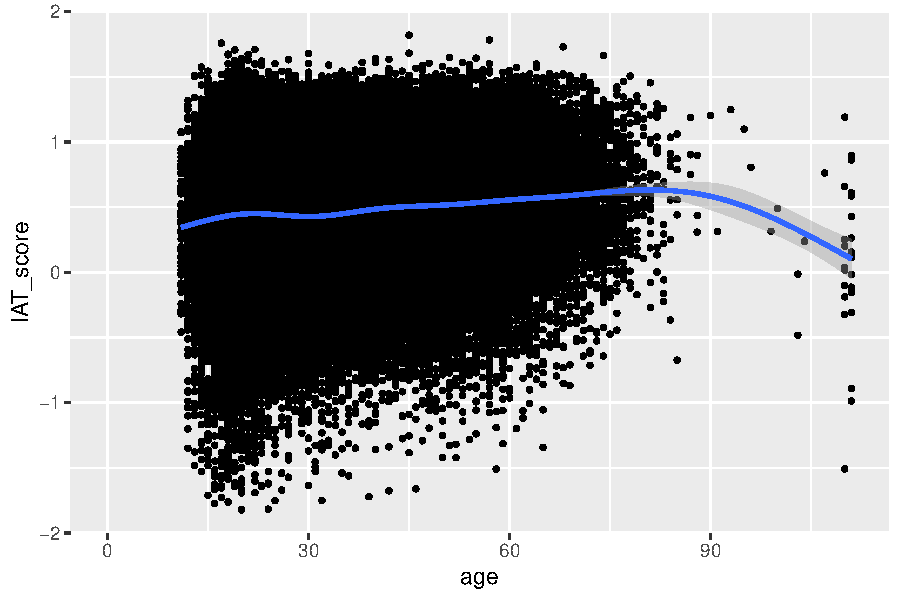
\includegraphics[keepaspectratio]{Lab_04_instructions_files/figure-pdf/unnamed-chunk-4-1.pdf}}
\end{center}

In the above scatterplot, it looks like the relationship is mostly
linear (and increasing) until we get to approximately 90 years old. At
that point IAT score decreases with age. Let's say we 100\% believe
there is suddenly more responders around 110 years old than 90-100 year
olds. I'm already skeptical of this since we did a quality control in
Lab 3. We'll play it out because it's not worth making judgement calls
on what we consider ``admissable'' data.

We could do quantiles, splines, or polynomials, but those approaches
will either make more categorical variables or make the relationship
between age and IAT score harder to interpret. We have a pretty linear
relationship up until the higher ages!

I wanted to investigate the linearity a little more so I created an
indicator for individuals who are 100 years or older:

\begin{Shaded}
\begin{Highlighting}[]
\NormalTok{iat1 }\OtherTok{=}\NormalTok{ iat }\SpecialCharTok{\%\textgreater{}\%} \FunctionTok{mutate}\NormalTok{(}\AttributeTok{ind\_age\_100 =} \FunctionTok{ifelse}\NormalTok{(age }\SpecialCharTok{\textgreater{}} \DecValTok{100}\NormalTok{, }\StringTok{"TRUE"}\NormalTok{, }\StringTok{"FALSE"}\NormalTok{))}
\end{Highlighting}
\end{Shaded}

Now I can see if the linearity differs between the two groups of ages:

\begin{Shaded}
\begin{Highlighting}[]
\FunctionTok{ggplot}\NormalTok{(iat1, }\FunctionTok{aes}\NormalTok{(}\AttributeTok{x =}\NormalTok{ age, }\AttributeTok{y =}\NormalTok{ IAT\_score, }\AttributeTok{color =}\NormalTok{ ind\_age\_100)) }\SpecialCharTok{+}
  \FunctionTok{geom\_point}\NormalTok{(}\AttributeTok{size =} \FloatTok{0.8}\NormalTok{) }\SpecialCharTok{+} \FunctionTok{geom\_smooth}\NormalTok{(}\AttributeTok{method =} \StringTok{"lm"}\NormalTok{)}
\end{Highlighting}
\end{Shaded}

\pandocbounded{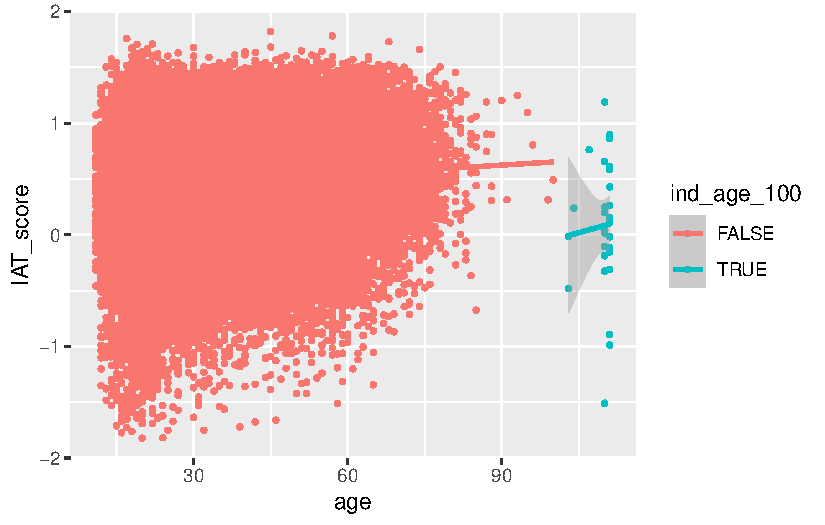
\includegraphics[keepaspectratio]{Lab_04_instructions_files/figure-pdf/unnamed-chunk-6-1.pdf}}

I am happy to see that both groups' IAT score are increasing with age.
It actually looks like my indicator might be a confounder\ldots{} In
that case, we only need to include the indicator in the model so that
the relationship between age and IAT is adjusted for the indicator. I
can test to see if the indicator is a big enough confoudner using the
change in coefficient of age and my explanatory variable.

Here's the model without the indicator:

\begin{Shaded}
\begin{Highlighting}[]
\NormalTok{prelim\_model }\OtherTok{=} \FunctionTok{lm}\NormalTok{(IAT\_score }\SpecialCharTok{\textasciitilde{}}\NormalTok{ iam\_unordered }\SpecialCharTok{+}\NormalTok{ identfat }\SpecialCharTok{+}\NormalTok{ comptomost }\SpecialCharTok{+} 
\NormalTok{                  ind\_m }\SpecialCharTok{+}\NormalTok{ ind\_f }\SpecialCharTok{+}\NormalTok{ ind\_tmm }\SpecialCharTok{+}\NormalTok{ ind\_twf }\SpecialCharTok{+}\NormalTok{ ind\_gqnc }\SpecialCharTok{+} 
\NormalTok{                    ind\_other }\SpecialCharTok{+}
\NormalTok{                  race }\SpecialCharTok{+} 
\NormalTok{                  ethn }\SpecialCharTok{+}
\NormalTok{                  edu\_14\_f }\SpecialCharTok{+}
\NormalTok{                  age, }\AttributeTok{data =}\NormalTok{ iat1)}
\end{Highlighting}
\end{Shaded}

And we'll take a look at the coefficients for the model:

\begin{Shaded}
\begin{Highlighting}[]
\NormalTok{prelim\_model}\SpecialCharTok{$}\NormalTok{coefficients[}\FunctionTok{c}\NormalTok{(}\DecValTok{2}\SpecialCharTok{:}\DecValTok{6}\NormalTok{, }\DecValTok{46}\NormalTok{)] }\CommentTok{\# by using c(2:6, 46) I am telling R to }
\end{Highlighting}
\end{Shaded}

\begin{verbatim}
      iam_unorderedVery underweight iam_unorderedModerately underweight 
                       -0.061151601                        -0.015513320 
  iam_unorderedSlightly underweight    iam_unorderedSlightly overweight 
                        0.006954580                        -0.023369363 
 iam_unorderedModerately overweight                                 age 
                       -0.056237038                         0.003857134 
\end{verbatim}

\begin{Shaded}
\begin{Highlighting}[]
                                      \CommentTok{\# only print certain variables\textquotesingle{} coefficients}
\end{Highlighting}
\end{Shaded}

Then we can run the model with the indicator, then look at the
coefficients:

\begin{Shaded}
\begin{Highlighting}[]
\NormalTok{prelim\_model2 }\OtherTok{=} \FunctionTok{lm}\NormalTok{(IAT\_score }\SpecialCharTok{\textasciitilde{}}\NormalTok{ iam\_unordered }\SpecialCharTok{+}\NormalTok{ identfat }\SpecialCharTok{+}\NormalTok{ comptomost }\SpecialCharTok{+} 
\NormalTok{                  ind\_m }\SpecialCharTok{+}\NormalTok{ ind\_f }\SpecialCharTok{+}\NormalTok{ ind\_tmm }\SpecialCharTok{+}\NormalTok{ ind\_twf }\SpecialCharTok{+}\NormalTok{ ind\_gqnc }\SpecialCharTok{+}\NormalTok{ ind\_other }\SpecialCharTok{+}
\NormalTok{                  race }\SpecialCharTok{+} 
\NormalTok{                  ethn }\SpecialCharTok{+}
\NormalTok{                  edu\_14\_f }\SpecialCharTok{+}
\NormalTok{                  age }\SpecialCharTok{+}\NormalTok{ ind\_age\_100, }
                 \AttributeTok{data =}\NormalTok{ iat1)}
\NormalTok{prelim\_model2}\SpecialCharTok{$}\NormalTok{coefficients[}\FunctionTok{c}\NormalTok{(}\DecValTok{2}\SpecialCharTok{:}\DecValTok{6}\NormalTok{, }\DecValTok{46}\NormalTok{)] }\CommentTok{\# by using c(2:6, 46) I am telling R to }
\end{Highlighting}
\end{Shaded}

\begin{verbatim}
      iam_unorderedVery underweight iam_unorderedModerately underweight 
                       -0.060385515                        -0.015352043 
  iam_unorderedSlightly underweight    iam_unorderedSlightly overweight 
                        0.006817642                        -0.023677757 
 iam_unorderedModerately overweight                                 age 
                       -0.056762301                         0.003918822 
\end{verbatim}

\begin{Shaded}
\begin{Highlighting}[]
                                       \CommentTok{\# only print certain variables\textquotesingle{} coefficients}
\end{Highlighting}
\end{Shaded}

We can check the \% change in the coefficients between the models.

Recall, \[
\Delta\% = 100\% \cdot \frac{\widehat\beta_{FLR, full} - \widehat\beta_{FLR, red}}{\widehat\beta_{FLR, full}}
\] Here's how I quickly do it with the coefficients:

\begin{Shaded}
\begin{Highlighting}[]
\DecValTok{100} \SpecialCharTok{*}\NormalTok{ ( prelim\_model2}\SpecialCharTok{$}\NormalTok{coefficients[}\FunctionTok{c}\NormalTok{(}\DecValTok{2}\SpecialCharTok{:}\DecValTok{6}\NormalTok{, }\DecValTok{46}\NormalTok{)] }\SpecialCharTok{{-}}\NormalTok{ prelim\_model}\SpecialCharTok{$}\NormalTok{coefficients[}\FunctionTok{c}\NormalTok{(}\DecValTok{2}\SpecialCharTok{:}\DecValTok{6}\NormalTok{, }\DecValTok{46}\NormalTok{)] ) }\SpecialCharTok{/}
\NormalTok{  prelim\_model2}\SpecialCharTok{$}\NormalTok{coefficients[}\FunctionTok{c}\NormalTok{(}\DecValTok{2}\SpecialCharTok{:}\DecValTok{6}\NormalTok{, }\DecValTok{46}\NormalTok{)]}
\end{Highlighting}
\end{Shaded}

\begin{verbatim}
      iam_unorderedVery underweight iam_unorderedModerately underweight 
                         -1.2686585                          -1.0505274 
  iam_unorderedSlightly underweight    iam_unorderedSlightly overweight 
                         -2.0085770                           1.3024639 
 iam_unorderedModerately overweight                                 age 
                          0.9253735                           1.5741387 
\end{verbatim}

Based on \%'s above, it doesn't look like the indicator makes much of a
difference in my model. It is likely because there are only 29
individuals over the age of 100 and 201,031 individuals under the age of
100 (In my dataset). Those 29 individuals will not have a big impact on
the linear relationship between age and IAT, even though the first
smoothed scatterplot made it look like it does.

To bring this point home, I can plot age and IAT with and without the
individuals that are 100 years or older. Let me know if you find a
better way to overlay these plots! (I have been a little stressed on
time, and couldn't find a quick answer.)

\begin{Shaded}
\begin{Highlighting}[]
\FunctionTok{ggplot}\NormalTok{(iat1, }\FunctionTok{aes}\NormalTok{(}\AttributeTok{x =}\NormalTok{ age, }\AttributeTok{y =}\NormalTok{ IAT\_score)) }\SpecialCharTok{+}
  \FunctionTok{geom\_point}\NormalTok{() }\SpecialCharTok{+} \FunctionTok{geom\_smooth}\NormalTok{(}\AttributeTok{method =} \StringTok{"lm"}\NormalTok{) }\SpecialCharTok{+} \FunctionTok{xlim}\NormalTok{(}\DecValTok{0}\NormalTok{, }\DecValTok{111}\NormalTok{) }\SpecialCharTok{+}
  \FunctionTok{labs}\NormalTok{(}\AttributeTok{title =} \StringTok{"With individuals 100 years or older"}\NormalTok{)}
\end{Highlighting}
\end{Shaded}

\pandocbounded{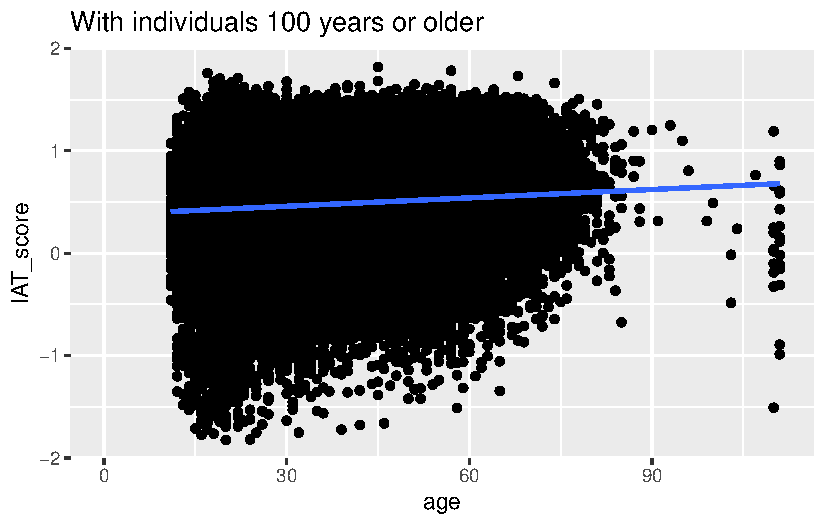
\includegraphics[keepaspectratio]{Lab_04_instructions_files/figure-pdf/unnamed-chunk-11-1.pdf}}

\begin{Shaded}
\begin{Highlighting}[]
\FunctionTok{ggplot}\NormalTok{(iat1 }\SpecialCharTok{\%\textgreater{}\%} \FunctionTok{filter}\NormalTok{(age }\SpecialCharTok{\textless{}} \DecValTok{100}\NormalTok{), }\FunctionTok{aes}\NormalTok{(}\AttributeTok{x =}\NormalTok{ age, }\AttributeTok{y =}\NormalTok{ IAT\_score)) }\SpecialCharTok{+}
  \FunctionTok{geom\_point}\NormalTok{() }\SpecialCharTok{+} \FunctionTok{geom\_smooth}\NormalTok{(}\AttributeTok{method =} \StringTok{"lm"}\NormalTok{) }\SpecialCharTok{+} \FunctionTok{xlim}\NormalTok{(}\DecValTok{0}\NormalTok{, }\DecValTok{111}\NormalTok{) }\SpecialCharTok{+}
  \FunctionTok{labs}\NormalTok{(}\AttributeTok{title =} \StringTok{"Without individuals 100 years or older"}\NormalTok{)}
\end{Highlighting}
\end{Shaded}

\pandocbounded{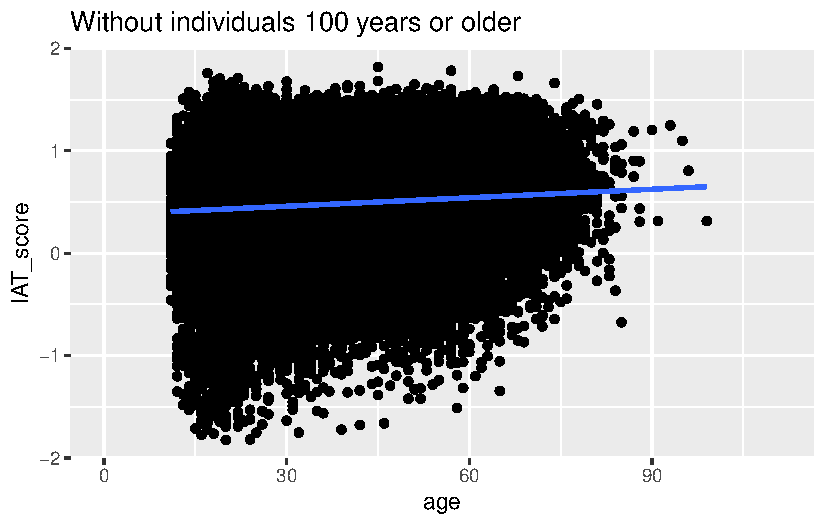
\includegraphics[keepaspectratio]{Lab_04_instructions_files/figure-pdf/unnamed-chunk-11-2.pdf}}

I see no difference. Thus, I think it's okay to leave age as is!!

\begin{tcolorbox}[enhanced jigsaw, leftrule=.75mm, coltitle=black, titlerule=0mm, opacityback=0, opacitybacktitle=0.6, bottomtitle=1mm, colbacktitle=quarto-callout-important-color!10!white, rightrule=.15mm, colframe=quarto-callout-important-color-frame, left=2mm, bottomrule=.15mm, toptitle=1mm, colback=white, title=\textcolor{quarto-callout-important-color}{\faExclamation}\hspace{0.5em}{Tasks}, arc=.35mm, breakable, toprule=.15mm]

No tasks here! If you want to try out what I did above, you can!

\end{tcolorbox}

\subsubsection{Step 5: Check for
interactions}\label{step-5-check-for-interactions}

Now we're going to check if there are any interactions. I will walk you
through a streamlined way to check for interactions between your
explanatory variable and all the other variables in the model.

First, I want you to revisit your work in Lab 3. Remind yourself of the
variables that you identified as possible effect modifiers.

As you check for interactions, don't forget to make your decisions
\textbf{based on your discussion/hypotheses in Lab 3}. Always prioritize
investigation of interactions that are justified clinically before
investigating interactions only based on statistical significance.

\phantomsection\label{annotated-cell-12}%
\begin{Shaded}
\begin{Highlighting}[]
\NormalTok{vars }\OtherTok{=} \FunctionTok{names}\NormalTok{(}\FunctionTok{model.frame}\NormalTok{(prelim\_model))[}\SpecialCharTok{{-}}\DecValTok{1}\NormalTok{] }\hspace*{\fill}\NormalTok{\circled{1}}

\NormalTok{.env }\OtherTok{\textless{}{-}} \FunctionTok{environment}\NormalTok{()}
\NormalTok{interactions }\OtherTok{\textless{}{-}} \FunctionTok{combn}\NormalTok{(vars, }\DecValTok{2}\NormalTok{, }\ControlFlowTok{function}\NormalTok{(x) }\FunctionTok{paste}\NormalTok{(x, }\AttributeTok{collapse=}\StringTok{" * "}\NormalTok{)) }\SpecialCharTok{\%\textgreater{}\%} \hspace*{\fill}\NormalTok{\circled{2}}
    \FunctionTok{grep}\NormalTok{(., }\AttributeTok{pattern =} \StringTok{"iam\_unordered"}\NormalTok{, }\AttributeTok{value =}\NormalTok{ T) }\hspace*{\fill}\NormalTok{\circled{3}}
\end{Highlighting}
\end{Shaded}

\begin{description}
\tightlist
\item[\circled{1}]
Create a vector of the variable names that are in your preliminary
model. Note I use \texttt{{[}-1{]}} to remove \texttt{IAT\_score} from
my list. Please make sure to change \texttt{prelim\_model} to the name
of your model at this point.
\item[\circled{2}]
Here we are just combining all our covariates into interactions that R
can understand. This makes it so we don't have to write it all
ourselves.
\item[\circled{3}]
Make sure to change the \texttt{pattern\ =\ "iam\_unordered"} to be
\texttt{pattern\ =} to your explanatory variable.
\end{description}

Now that we've created the set up for all the possible interactions, we
can run them through the \texttt{lm()} function and see the summary of
the models. In the following code I use the \texttt{lappy()} function to
fit an individual model for the main effects + each interaction listed
in \texttt{interactions}.

\begin{tcolorbox}[enhanced jigsaw, leftrule=.75mm, coltitle=black, titlerule=0mm, opacityback=0, opacitybacktitle=0.6, bottomtitle=1mm, colbacktitle=quarto-callout-note-color!10!white, rightrule=.15mm, colframe=quarto-callout-note-color-frame, left=2mm, bottomrule=.15mm, toptitle=1mm, colback=white, title=\textcolor{quarto-callout-note-color}{\faInfo}\hspace{0.5em}{Note}, arc=.35mm, breakable, toprule=.15mm]

Please note that this code takes a while to run. Once you run it and
take note of the results, you can comment out or add
\texttt{\#\textbar{}\ eval:\ false} to prevent it from running every
time you render. You don't need to show the results for this in your
submitted work, but I want to see the code, and read about your
decisions about from results.

\end{tcolorbox}

\begin{Shaded}
\begin{Highlighting}[]
\NormalTok{summary }\OtherTok{=} \FunctionTok{lapply}\NormalTok{(interactions,}
             \ControlFlowTok{function}\NormalTok{(int) }\FunctionTok{summary}\NormalTok{(}\FunctionTok{lm}\NormalTok{(}\FunctionTok{reformulate}\NormalTok{(}\FunctionTok{c}\NormalTok{(vars, int), }\StringTok{"IAT\_score"}\NormalTok{, }\AttributeTok{env=}\NormalTok{.env),}
                                      \AttributeTok{data =}\NormalTok{ iat)))}
\NormalTok{summary}
\end{Highlighting}
\end{Shaded}

You can alse go straight to using the \texttt{anova()} function to
compare the preliminary model.

\phantomsection\label{annotated-cell-14}%
\begin{Shaded}
\begin{Highlighting}[]
\NormalTok{anova\_res }\OtherTok{=} \FunctionTok{lapply}\NormalTok{(interactions,}
             \ControlFlowTok{function}\NormalTok{(int) }\FunctionTok{anova}\NormalTok{(}\FunctionTok{lm}\NormalTok{(}\FunctionTok{reformulate}\NormalTok{(}\FunctionTok{c}\NormalTok{(vars, int), }\StringTok{"IAT\_score"}\NormalTok{, }\AttributeTok{env=}\NormalTok{.env),}
                                      \AttributeTok{data =}\NormalTok{ iat),}
\NormalTok{                                 prelim\_model)) }\hspace*{\fill}\NormalTok{\circled{1}}
\NormalTok{anova\_res[}\DecValTok{1}\NormalTok{]}
\NormalTok{g }\OtherTok{=}\NormalTok{ anova\_res[[}\DecValTok{1}\NormalTok{]]}
\NormalTok{g}\SpecialCharTok{$}\NormalTok{F}
\end{Highlighting}
\end{Shaded}

\begin{description}
\tightlist
\item[\circled{1}]
You will to change this name for the preliminary model if you called it
something different.
\end{description}

\begin{verbatim}
[[1]]
Analysis of Variance Table

Model 1: IAT_score ~ iam_unordered + identfat + comptomost + ind_m + ind_f + 
    ind_tmm + ind_twf + ind_gqnc + ind_other + race + ethn + 
    edu_14_f + age + iam_unordered * identfat
Model 2: IAT_score ~ iam_unordered + identfat + comptomost + ind_m + ind_f + 
    ind_tmm + ind_twf + ind_gqnc + ind_other + race + ethn + 
    edu_14_f + age
  Res.Df   RSS  Df Sum of Sq     F    Pr(>F)    
1 200990 31337                                  
2 201014 31346 -24   -9.4223 2.518 5.558e-05 ***
---
Signif. codes:  0 '***' 0.001 '**' 0.01 '*' 0.05 '.' 0.1 ' ' 1

[1]       NA 2.518048
\end{verbatim}

\begin{tcolorbox}[enhanced jigsaw, leftrule=.75mm, coltitle=black, titlerule=0mm, opacityback=0, opacitybacktitle=0.6, bottomtitle=1mm, colbacktitle=quarto-callout-important-color!10!white, rightrule=.15mm, colframe=quarto-callout-important-color-frame, left=2mm, bottomrule=.15mm, toptitle=1mm, colback=white, title=\textcolor{quarto-callout-important-color}{\faExclamation}\hspace{0.5em}{Tasks}, arc=.35mm, breakable, toprule=.15mm]

Using your discussion in Lab 3 and the results from the F-test on
interactions:

\begin{enumerate}
\def\labelenumi{\arabic{enumi}.}
\tightlist
\item
  Create a list of the interactions that you will include in your model.
\item
  Run the preliminary final model that includes the main effects and
  interactions.
\end{enumerate}

\end{tcolorbox}

\subsubsection{Step 6: Assess model fit}\label{step-6-assess-model-fit}

At this point we may want to compare different models. While Steps 1-5
have been directing us towards a single model, you may have been
interested in other models along the way. Maybe there were some
interactions that you thought were interesting, but didn't think of
before. Maybe you would like to combine different groups for categorical
variables.

If you are completely happy with your model, then you don't have to do
this step.

You might create a table like such:

\begin{Shaded}
\begin{Highlighting}[]
\NormalTok{sum }\OtherTok{=} \FunctionTok{summary}\NormalTok{(prelim\_model)}
\NormalTok{model\_fit\_stats }\OtherTok{=} \FunctionTok{data.frame}\NormalTok{(}\AttributeTok{Model =} \StringTok{"Preliminary main effects model"}\NormalTok{,}
                             \AttributeTok{Adjusted\_R\_sq =}\NormalTok{ sum}\SpecialCharTok{$}\NormalTok{adj.r.squared, }
                             \AttributeTok{AIC =} \FunctionTok{AIC}\NormalTok{(prelim\_model), }
                             \AttributeTok{BIC =} \FunctionTok{BIC}\NormalTok{(prelim\_model))}

\NormalTok{model\_fit\_stats}
\end{Highlighting}
\end{Shaded}

\begin{verbatim}
                           Model Adjusted_R_sq      AIC      BIC
1 Preliminary main effects model    0.04511326 197006.6 197486.5
\end{verbatim}

\begin{tcolorbox}[enhanced jigsaw, leftrule=.75mm, coltitle=black, titlerule=0mm, opacityback=0, opacitybacktitle=0.6, bottomtitle=1mm, colbacktitle=quarto-callout-important-color!10!white, rightrule=.15mm, colframe=quarto-callout-important-color-frame, left=2mm, bottomrule=.15mm, toptitle=1mm, colback=white, title=\textcolor{quarto-callout-important-color}{\faExclamation}\hspace{0.5em}{Tasks}, arc=.35mm, breakable, toprule=.15mm]

\textbf{Optional:} Create a table that displays some fo the model fit
statistics to compare preliminary final models.

\end{tcolorbox}

\subsubsection{Create a forest plot of your coefficient
estimates}\label{create-a-forest-plot-of-your-coefficient-estimates}

It's often helpful to have a visualization of coefficient estimates.
Forest plots are a nice way to show all the values together. Below I
have started a forest plot using my \texttt{prelim\_model}. You can make
the plot with your final model.

I used the \texttt{plot\_model()} function to make the plot, and
\href{https://cran.r-project.org/web/packages/sjPlot/vignettes/plot_model_estimates.html}{here's
a site} that discusses some of it's capabilities. The below plot is just
a starting point!! You'll need to clean up the variables, title, etc.

You may use another function to make the plots. I chose this one since
it can handle the model as input.

\begin{Shaded}
\begin{Highlighting}[]
\FunctionTok{plot\_model}\NormalTok{(prelim\_model, }\AttributeTok{show.values =} \ConstantTok{TRUE}\NormalTok{, }\AttributeTok{value.offset =} \FloatTok{0.5}\NormalTok{) }\SpecialCharTok{+} \FunctionTok{ylim}\NormalTok{(}\SpecialCharTok{{-}}\FloatTok{0.25}\NormalTok{, }\FloatTok{0.25}\NormalTok{)}
\end{Highlighting}
\end{Shaded}

\begin{verbatim}
Scale for y is already present.
Adding another scale for y, which will replace the existing scale.
\end{verbatim}

\begin{center}
\pandocbounded{\includegraphics[keepaspectratio]{Lab_04_instructions_files/figure-pdf/unnamed-chunk-16-1.pdf}}
\end{center}

Here are some other packages for forest plots:

\begin{itemize}
\tightlist
\item
  https://cran.r-project.org/web/packages/forestploter/vignettes/forestploter-intro.html
\item
  https://larmarange.github.io/ggstats/articles/ggcoef\_model.html
\end{itemize}

\begin{tcolorbox}[enhanced jigsaw, leftrule=.75mm, coltitle=black, titlerule=0mm, opacityback=0, opacitybacktitle=0.6, bottomtitle=1mm, colbacktitle=quarto-callout-important-color!10!white, rightrule=.15mm, colframe=quarto-callout-important-color-frame, left=2mm, bottomrule=.15mm, toptitle=1mm, colback=white, title=\textcolor{quarto-callout-important-color}{\faExclamation}\hspace{0.5em}{Tasks}, arc=.35mm, breakable, toprule=.15mm]

Create a forest plot \textbf{or regression table} to visualize the
coefficient estimates.

\end{tcolorbox}




\end{document}
